\subsection{Guatemala}\label{subsec:gua}

In Guatemala the site is located at the top of the roof of the T1 building of
the University of San Carlos de Guatemala. The size of the detector is 1.2\,m
height, 1.12\,m wide and has a capacity of 1,100\,l. The inside is coated
with a reflective Flex polyvinyl chloride sheet and the PMT is a 9" photonis
XP1802.

The electronic of the detector is the original from the Bariloche groupand was
running from June 2011 until March 2012.


\begin{figure}[h]
\begin{center}
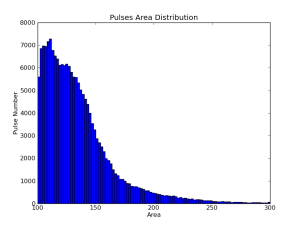
\includegraphics[width=0.48\textwidth]{images/guatemala/Histo.png}
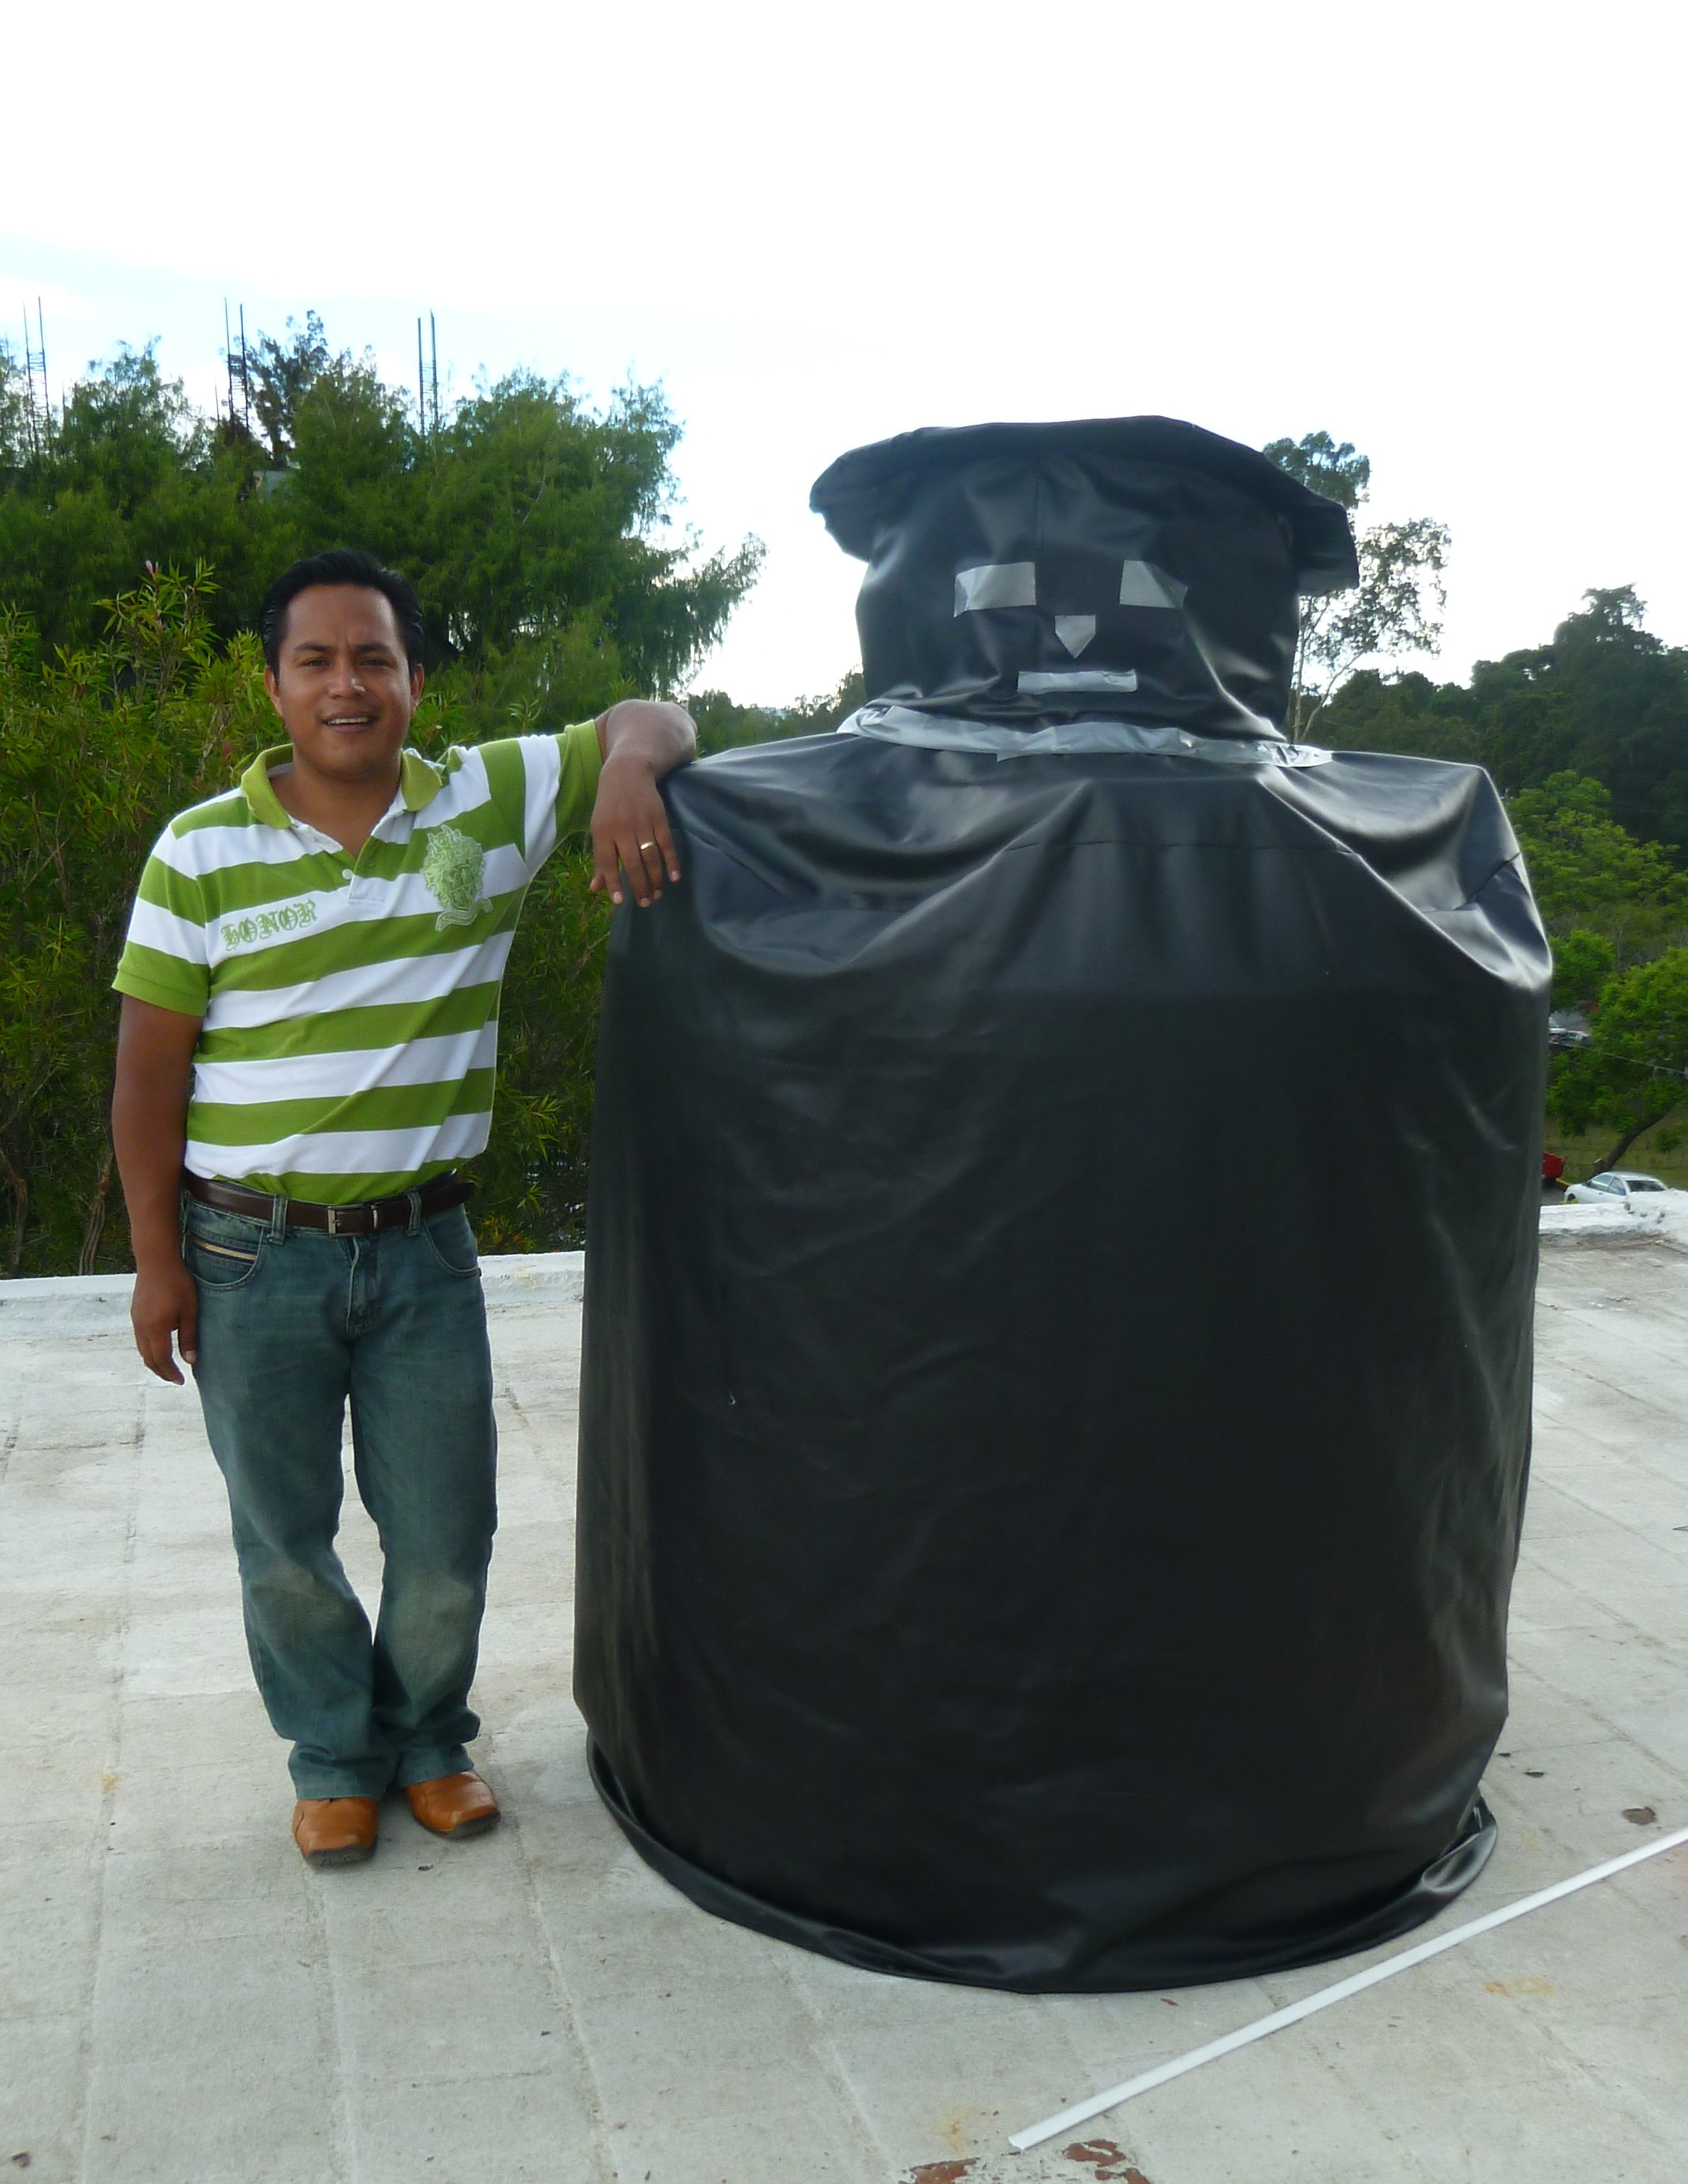
\includegraphics[width=0.48\textwidth]{images/guatemala/DimDet.jpg}
\caption{Histogram of an event of the uncalibrated detector. The area is proportional to the charge recolected. The second peak corresponds to a muonic trace.The entire detector is covered with black semi-leather.}
\label{fig:Histo-guate} 
\end{center}
\end{figure}
